\chapter{Arquitetura do Software}
\thispagestyle{empty} % retira numeracao da pagina, conforme as normas de apresentacao.

A implementação do projeto ocorreu em um contexto cliente-servidor, ou seja, foram desenvolvidas duas aplicações. A primeira, realizada no \textit{server side}, ou lado do servidor, consistiu no desenvolvimento de um sistema \textit{web} que funciona como uma API. Este sistema tem como objetivo receber requisições da aplicação implementada no \textit{client-side}, ou lado do cliente, e se comunicar com as API's das LMS's, obtendo as informações referentes ao usuário, como por exemplo as suas disciplinas. O sistema também é responsável por adaptar tais informações para o formato suportado pela aplicação cliente antes de enviá-las. Já a aplicação do lado do cliente foi desenvolvida como um aplicativo móvel, e tem como responsabilidade prover uma interface simples de usar e que reúna e apresente todas as informações dos sistemas LMSs integrados em um único local.

\section{\textit{Server-Side}}
							
Para o desenvolvimento da aplicação do servidor foi utilizada a linguagem de programação \textit{Ruby} 
(MATSUMOTO, 1995), orientada a objetos, interpretada e com foco na produtividade e simplicidade além de ser totalmente livre. 

Em conjunto foi o utilizado o \textit{Ruby On Rails}, um \textit{framework web}. Criado com \textit{Ruby}, seu objetivo é tornar o desenvolvimento \textit{web} o mais simples possível. Trazendo consigo todo o necessário para construir uma aplicação moderna. Ele possui as seguintes características:

\begin{itemize}
    \item COC (\textit{Convention Over Configuration}, ou Convenção Sobre Configuração): um paradigma que busca determinar um padrão de regras e organização em busca de diminuir o número de decisões e configurações que o desenvolvedor precisa realizar para iniciar o desenvolvimento.
    
    \item RESTFul (\textit{Representational State Transfer}, ou Transferência do Estado Representacional):de acordo com Fielding (2000), consiste no uso de identificadores de recurso (URL) e a mudanç̧a de estados de um objeto utilizando métodos do protocolo HTTP, como os métodos \textit{GET}, \textit{POST}, \textit{PUT} e \textit{DELETE}.
\end{itemize}

A estrutura de uma aplicação Rails é o padrão MVC (Modelo-Visão-Controlador) que organiza a lógica de programação em três camadas principais. O modelo, no qual colocamos a lógica de negócio. O controlador que recebe as interações ou requisições, direciona comandos ao modelo para enfim construir uma resposta HTML ou JSON como a visão. 

Considerando que novos sistemas de gerenciamento de ensino poderiam ser adicionados futuramente, tais integrações foram organizadas em uma estrutura de módulos. Na qual todo o código e lógica envolvida na integração de uma LMS específica foi encapsulado em um módulo isolado.

Contudo, ainda foi necessário a implementação de dois padrões de projeto adicionais na aplicação. Os padrões \textit{Adapter} (GAMMA et al., 1994) e \textit{Strategy} (GAMMA et al., 1994) se mostraram muito úteis para que fosse possível alcançar os objetivos do sistema.
						
\subsection{Padrão \textit{Adapter}}

A intenção do padrão \textit{Adapter}, também conhecido como \textit{Wrapper}, é converter uma interface para outra interface diferente a qual é esperada pelo cliente. Ou seja, ele permite a comunicação de interfaces incompatíveis.	 	

\begin{figure}[H]
    \centering
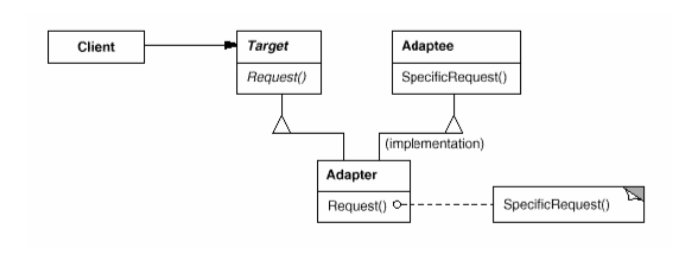
\includegraphics[scale=0.65]{5_1}
    \caption{Padrão \textit{Adapter}}
    \label{figura1}
\end{figure}
			
O padrão é importante para o projeto pois é necessário adaptar as diversas respostas obtidas das diferentes interfaces de cada uma das LMSs integradas ao sistema, para que seja possível que a interface cliente os utilize. Sendo assim, foram implementados um \textit{adapter} para cada recurso diferente previsto na aplicação.

\begin{itemize}
    \item \textit{CourseAdapter}: para disciplinas e cursos;
    \item \textit{EventAdapter}: para eventos;
    \item \textit{FileAdapter}: para arquivos;
    \item \textit{TopicAdapter}: para tópicos;
    \item \textit{AuthenticationAdapter}: responsável pela autenticação em cada um dos serviços integrados;
\end{itemize}

Sozinho este padrão não solucionava todo o problema. Como é preciso lidar com diversas interfaces diferentes, uma para cada LMS, tais classes precisariam ser modificadas toda vez que um sistema LMS novo fosse integrado. Pensando nisso, os \textit{adapters} foram combinados com um outro padrão, o \textit{Strategy}, que passa a cuidar da lógica de adaptação. Os \textit{adapters} recebem como parâmetro a LMS e define a \textit{strategy} correta para adaptação.

\subsection{Padrão \textit{Strategy}}

A intenção do padrão \textit{Strategy}, também conhecido como \textit{Policy}, é definir um grupo de algorítimos, encapsular cada um deles, e permitir que eles sejam permutáveis. Ou seja, permite que a lógica varie dependendo do cliente que precisa utilizá-la.	

\begin{figure}[H]
    \centering
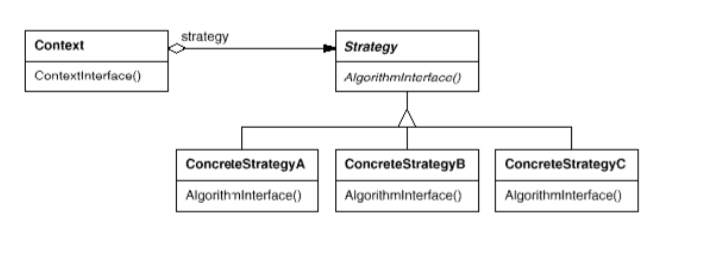
\includegraphics[scale=0.65]{5_2}
    \caption{Padrão \textit{Strategy}}
    \label{figura2}
\end{figure}

As \textit{strategies} do projeto foram idealizadas para serem implementadas isoladamente em cada módulo dos serviços integrados. E assim as classes \textit{adapters} poderíam trocar as estratégias de adaptação das interfaces baseado na chamada do cliente. Por isso, para cada um dos módulos foi preciso implementar uma \textit{policy} para cada recurso, da mesma forma que os adaptadores.

\begin{itemize}
    \item \textit{CourseStrategy}: para disciplinas e cursos;
    \item \textit{EventStrategy}: para eventos;
    \item \textit{FileStrategy}: para arquivos;
    \item \textit{TopicStrategy}: para tópicos;
    \item \textit{AuthenticationStrategy}: para a autenticação;
\end{itemize}


\section{Client-side}
\label{sec:client-side}
A aplicação Client-Side, isto é, a parte que será executada no dispositivo móvel do usuário, tem a função de apresentar de forma clara e objetiva as informações trazidas do \textit{Server-Side} através de uma interface de usuário que seja responsiva aos estímulos particulares utilizados em dispovitivos móveis, como o toque na tela, o arraste de objetos e a rolagem do conteúdo com gestos de "puxar" e "empurrar" dos dedos.  Além disso, a disposição do conteúdo deve levar em consideração o tamanho reduzido das telas dos dispositivos, os botões e teclas físicas disponíveis nos diversos tipos de aparelhos, bem como a disponibilidade e o meio de conectividade com a Internet.

Quando se fala de desenvolvimento de aplicativos para plataformas móveis, certamente um dos maiores desafios é lidar com a heterogeneidade em diversos aspectos dos dispositivos alvo. A começar pelo Hardware, temos telas que variam de 3 a 11 polegadas, com resoluções de imagem e densidades de pixels diversas, há também uma vasta gama de tecnologias de rede em padrões sortidos, com grandes variações nas taxas de transferência de dados, partindo dos 14kbps de conexões GPRS até  taxas superiores a 20Mbps em tecnologias como LTE e WiMax. Existem ainda muitos outros fatores importantes, como a capacidade e o tipo de mídia de armazenamento disponível, a quantidade e disposição dos botões físicos e funções correspondentes dentre os distintos fabricantes, a infindável variedade de hardwares de geolocalizadores, acelerômetros, bússulas, câmeras, entre outros.

A julgar pela diversidade apresentada no hardware já se pode constatar a necessidade de um ferramental próprio para lidar com este desafio. No entanto, divergências mais impactantes são apresentadas quando olhamos a fundo as possibilidades existentes na camada de Software dos dispositivos.
Analisando apenas as possibilidades de sistemas operacionais, constatamos a existência de uma grande quantidade de opções, sendo as principais o Android, o iOS, o Windows Phone \cite{report:idc}, além de outras distribuições menos representativas, ou que já perderam grande parte do seu mercado ao longo da última década, como Symbian, Blackberry e WebOS. 

Cada um dos Sistemas Operacionais traz junto consigo uma série de particularidades que devem ser consideradas ao ser escolhida como alvo de um projeto de aplicativo.
De todas essas particularidades, o tamanho da comunidade de usuários que será contemplada certamente exerce grande influência na escolha do Sistema Operacional que executará o aplicativo.
Outro grande fator a ser considerado é a plataforma de desenvolvimento associada, cada qual com suas respectivas linguagens e ambientes de programação de diferentes custos de propriedade, suas respectivas lojas, custos e regras de distribuição impostos pelos seus fabricantes.


Foi necessário uma análise entre os tipos de aplicativo móvel possíveis de ser desenvolvidos para contornar o problema da alta heterogeneidade dos dispositivos de forma que fosse possível oferecer, com custo de desenvolvimento e qualidade satisfatórios, o aplicativo para a maior parcela possível de usuários dentro da comunidade alvo do projeto. Abordaremos estes diferentes tipos de aplicativo e exploraremos suas vantagens e desvantagens na sessão seguinte e apresentaremos a solução encontrada para o problema relatado.


\subsection{Abordagens de desenvolvimento de Aplicativo Móvel}

\begin{itemize}
    \item Aplicativos Nativos - São específicos para uma determinada plataforma móvel, como iOS ou Android, são construídos diretamente sobre os serviços disponibilizados pela plataforma móvel, expostos através de um conjunto de \textit{Interfaces de Programação de Aplicação (API)} \cite{book:fling}. Utilizam as ferramentas de desenvolvimento e linguagem específicas que as respectivas plataformas suportam \cite{article:malovolta}. Por exemplo, Xcode e Objective-C são suportadas pelo fabricante para desenvolver para iOS, e o Eclipse e a linguagem de programação Java são recomendados para o desenvolvimento para Android. Aplicativos nativos acessam geralmente executam de forma mais fluída por ter melhor desempenho no acesso às funções nativas do dispositivo \cite{article:corral}. Podem trazer uma sensação de usabilidade mais prazerosa, especialmente para requisitos de alto desempenho, como aceleração gráfica por hardware e leitura de sensores em sistemas de tempo real.
    \item Aplicativos Web ou Webapps: Usam as tecnologias web padrão, HTML5, JavaScript e CSS \cite{article:rahul}. Nesta abordagem escreve-se o código uma única vez e o aplicativo pode ser executado em qualquer plataforma. Apesar dos desenvolvedores poderem criar aplicativos sofisticados com apenas HTML5 e JavaScript, existem algumas limitações vitais \cite{article:rahul}\cite{article:spyros}, especificamente o armazenamento offline seguro e o acesso às funcionalidades nativas dos dispositivos, como câmera, calendário, contatos, sensores, hardware de geolocalização, etc.
    \item Aplicativos Híbridos: Esta proposta torna possível incorporar Aplicativos Web dentro de uma fina camada recipiente nativa, combinando os elementos dos Aplicativos nativos e Webapps. A maior parte do aplicativo é construído usando tecnologias web compatíveis com todas plataformas, tais como HTML5, CSS e Javascript - as mesmas línguas usadas para escrever aplicativos web. No entanto, algum código nativo é utilizado para permitir que o aplicativo acesse funcionalidades mais específicas do dispositivo e produza uma experiência de usuário mais refinada. A vantagem desta abordagem é clara: apenas uma porção do código nativo tem de ser re-escrito para o aplicativo funcionar adequadamente sobre os diferentes tipos de dispositivos disponíveis \cite{book:wargo}, se tornando mais rápido e mais fácil de desenvolver que aplicativos nativos \cite{article:ibm}.
\end{itemize}

\pagebreak

\begin{table}[h]
\centering
\caption{Vantagens das abordagens de desenvolvimento de aplicativos móveis \cite{article:swot}}
\begin{tabular}{p{.10\textwidth}|p{.90\textwidth}}
Web & \begin{minipage}{5in}
      \vskip 4pt
      \begin{itemize}
        \item Capacidade de construir uma única vez e implantar todas plataformas
        \item Distribuição Centralizada
      \end{itemize}
      \vskip 4pt
    \end{minipage} \\ \hline
Híbrido & \begin{minipage}{5in}
      \vskip 4pt
      \begin{itemize}
        \item Capacidade de construir uma única vez e implantar todas plataformas
        \item  Custos de desenvolvimento e manutenção reduzidos
        \item Tempo de lançamento reduzido\\ Segurança e gestão do aplicativo aprimorados\\ Desenvolvimento por pessoas com a mesma experiência (HTML5, CSS3, JavaScript)
        \item Acesso as APIs Nativas\\ Distribuição por Loja de Aplicativos
        \item Processamento impulsionado pelo hardware do dispositivo
        \end{itemize}
      \vskip 4pt
    \end{minipage} \\ \hline
Nativo & \begin{minipage}{5in}
      \vskip 4pt
      \begin{itemize}
        \item Melhor desempenho
        \item Rápida adaptação para mudanças no sistema operacional
        \item Controle total do dispositivoSegurança e Gestão de Aplicativos Aprimorados
        \item Acesso as APIs Nativas
        \item Distribuição por Loja de Aplicativos
        \item Processamento impulsionado pelo hardware do dispositivo
      \end{itemize}
      \vskip 4pt
    \end{minipage}
\end{tabular}
\end{table}

\pagebreak




\begin{table}[h]
\centering
\caption{Desvantagens das abordagens de desenvolvimento de aplicativos móveis \cite{article:swot}}
\begin{tabular}{p{.10\textwidth}|p{.90\textwidth}}
\multicolumn{1}{r|}{Web} & \begin{minipage}{5in}
      \vskip 4pt
      \begin{itemize}
        \item Sem acesso as APIs nativas
        \item Sem modo Offline
        \item Processamento não pode ser impulsionado pelo hardware do dispositivo
        \end{itemize}
      \vskip 4pt
    \end{minipage} \\ \hline
Híbrido & \begin{minipage}{5in}
      \vskip 4pt
      \begin{itemize}
        \item Funções nativas específicas podem estar ausentes em algumas plataformas e exigir codificação nativa
        \item Adaptação lenta a mudanças do sistema operacional
        \item Inadequado para requisitos de alta performance
        \end{itemize}
      \vskip 4pt
    \end{minipage} \\ \hline
Nativo & \begin{minipage}{5in}
      \vskip 4pt
      \begin{itemize}
        \item Cada plataforma requer o desenvolvimento independente por times de diferentes especialidades técnicas
        \item Requer teste de plataforma específico
        \item Suporte reduzido e menor oferta de desenvolvedores dependendo da plataforma
        \end{itemize}
      \vskip 4pt
    \end{minipage}
\end{tabular}
\label{my-label}
\end{table}

Considerando o escopo das funcionalidades do aplicativo proposto por este projeto, foi constatado que a maior parte das funcionalidades são relativas a apresentação de conteúdo e que não demandam recursos de alto desempenho para seu bom funcionamento \cite{article:malovolta2}. Soma-se a esta constatação, que promover o acesso a maior parcela possível da comunidade alvo é de suma importância para a proposta deste projeto, portanto todas as plataformas majoritárias devem poder ser atendidas. Por último, é desejavel que alguns recursos nativos estejam disponíveis, como sincronização de informações de acordo com o tipo de conexão disponível, notificações do dispositivo para alertar sobre novos conteúdos e acesso ao sistema de arquivos para armazenamento automático de materiais disponibilizados no aplicativo. Desta forma, a solução Híbrida é a opção mais adequada para a implementação da proposta.

Dentre as tecnologias disponíveis para desenvolvimento móvel híbrido, a ferramenta escolhida para este trabalho, pela sua facilidade de uso, menor custo de desenvolvimento \cite{article:ibm} e que contempla os requisitos desejados é o framework de desenvolvimento móvel, Ionic.


\subsection{Framework de desenvolvimento móvel Ionic}

Para a implementação do aplicativo foi utilizada as largamente difundidas tecnologias WEB tradicionais, o HTML5, o CSS e a linguagem de programação Javascript.

Para que o aplicativo possa ser disponibilizado através de pacotes compilados para dispositivos móveis de diferentes plataformas, como iOS, Android ou Windows, foi utilizado o framework de desenvolvimento de aplicativos móveis híbridos Ionic.

O Ionic incorpora e integra outras tecnologias bastante populares no desenvolvimento web e móvel. Destacaremos dentre elas as seguintes:

\begin{itemize}
    \item O Apache Cordoba, responsável por intermediar o acesso da aplicação escrita em Javascript aos recursos nativos do aparelho, como sistema de arquivos, wi-fi, rede móvel, geolocalização, entre outros.
    \item O AngularJS, um framework Javascript para execução de Single Page Applications, construídas sobre o padrao Model-View-ViewModel
\end{itemize}

A seguir apresentaremos os conceitos chaves destas partes e como elas interagem entre si.



\subsection{\textit{Apache Cordova}}
O \textit{Apache Cordoba} é o \textit{framework} de desenvolvimento de aplicativos móveis híbridos mais popular da atualidade \cite{article:palmiere}, foi criado em 2008 pela Nitobi sob o nome de Phonegap, posteriormente adquirido pela Adobe. A ferramenta cria uma camada recipiente nativa, como uma "casca", para aplicativos escritos em tecnologias Web tradicionais com a finalidade de construir um  aplicativo multi-plataforma.
Com o Apache Cordova é possível gerar um único \textit{baseline}, ou seja escrever um único código-fonte e compilar para todas as principais plataformas, como Android, iOS, Windows Phone , Blackberry, dentre outras.
O código nativo gerado pelo Apache Cordova, permite chamadas aos recursos nativos dos dispositivos nas diversas plataformas de forma otimizada [Apache, Cordova], sem a necessidade de conhecer as interfaces nativas específicas de cada plataforma ou codificar em sua linguagem nativa, como Objective-C ou Java, por exemplo, podendo assim reduzir os custos do projeto \cite{article:tian}.

A arquitetura por trás do Apache Cordova é apresentada na figura \ref{cordova}. 

Na tabela \ref{recursos_suportados_cordova} podemos ver todos os recursos suportados atualmente pelo Apache Cordoba nas diversas plataformas

\begin{figure}[H]
\centering
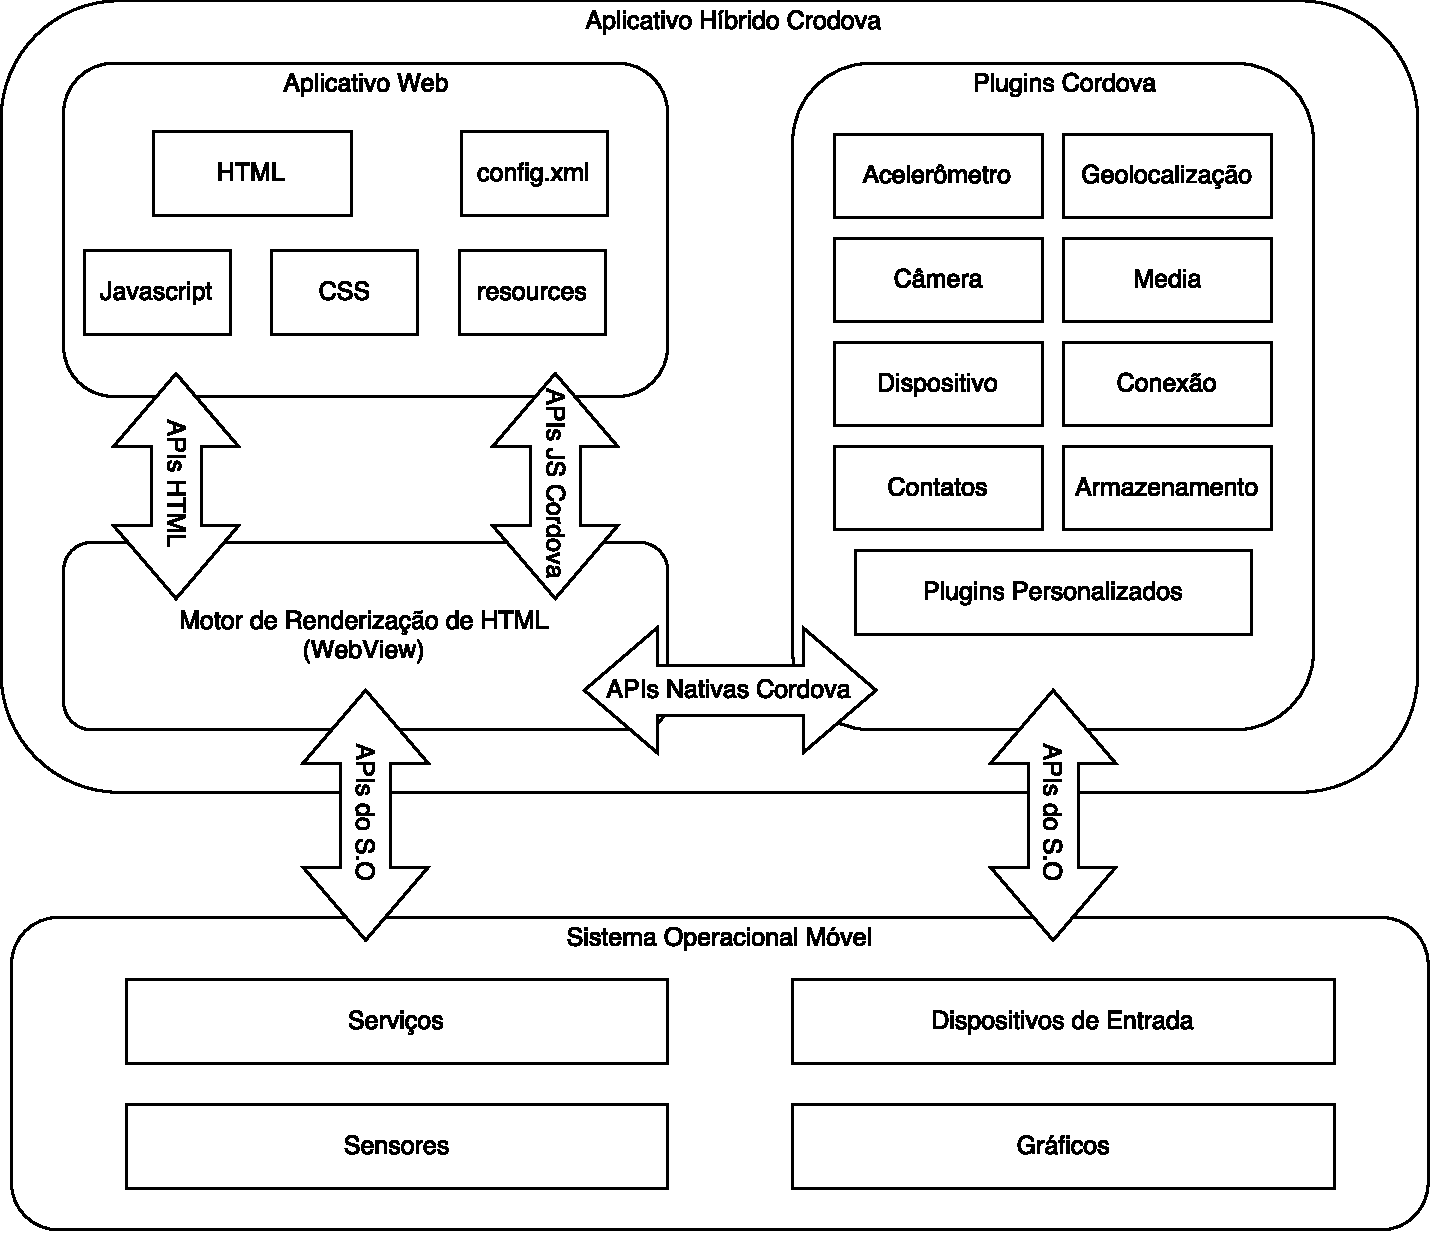
\includegraphics[width=\textwidth]{5_3.pdf}
    \caption{Arquitetura de uma aplicação híbrida com o Apache Cordova. \cite{website:cordova-arch}}
    \label{cordova}
\end{figure}



\begin{table}[h]
\resizebox{\textwidth}{!}{%
\centering
\begin{threeparttable}
\caption{Recursos suportados pela camada nativa do Apache Cordova \cite{website:cordova-platform}}
\label{recursos_suportados_cordova}
\begin{tabular}{rcccccc}
 & Android & Blackberry10 & iOS & Ubuntu & WP8 & Windows(8.1, 10, Phone 8.1) \\
Acelerômetro & \cmark & \cmark & \cmark & \cmark & \cmark & \cmark \\
Situação da Bateria & \cmark & \cmark & \cmark & \xmark & \cmark & \cmark ** \\
Câmera & \cmark & \cmark & \cmark & \cmark & \cmark & \cmark \\
Captura & \cmark & \cmark & \cmark & \cmark & \cmark & \cmark \\
Bússola & \cmark & \cmark & \cmark ** & \cmark & \cmark & \cmark \\
Conexão & \cmark & \cmark & \cmark & \cmark & \cmark & \cmark \\
Contatos & \cmark & \cmark & \cmark & \cmark & \cmark & \cmark * \\
Dispositivo & \cmark & \cmark & \cmark & \cmark & \cmark & \cmark \\
Eventos & \cmark & \cmark & \cmark & \cmark & \cmark & \cmark \\
Arquivos & \cmark & \cmark & \cmark & \cmark & \cmark & \cmark \\
Transferência de Arquivos & \cmark & \cmark * & \cmark & \xmark & \cmark * & \cmark * \\
Geolocalização & \cmark & \cmark & \cmark & \cmark & \cmark & \cmark \\
Globalização & \cmark & \cmark & \cmark & \cmark & \cmark & \cmark \\
Navegador Interno & \cmark & \cmark & \cmark & \cmark & \cmark & \cmark * \\
Media & \cmark & \cmark & \cmark & \cmark & \cmark & \cmark \\
\xmarkification & \cmark & \cmark & \cmark & \cmark & \cmark & \cmark \\
\textit{Splashscreen} & \cmark & \cmark & \cmark & \cmark & \cmark & \cmark \\
Barra de \textit{Status} & \cmark & \xmark & \cmark & \xmark & \cmark & \cmark ** \\
Armazenamento & \cmark & \cmark & \cmark & \cmark & \cmark * & \cmark * \\
Vibração & \cmark & \cmark & \cmark & \xmark & \cmark & \cmark **
\end{tabular}
    \begin{tablenotes}
          \begin{itemize}
              \item[\cmark] 
              suportado
              \item[\cmark*] 
              suportado com limitações
              \item[\cmark**] 
              suportado em algumas versões do S.O. 
              \item[\xmark]  
              não suportado
          \end{itemize}
    \end{tablenotes}
\end{threeparttable}
%
}
\end{table}
 
 
\pagebreak
 
\subsection{AngularJS}

AngularJS \cite{website:guidebook} é um framework Javascript de código aberto patrocinado e mantido pelo Google.
"O objetivo do AngularJS é trazer as ferramentas e recursos que estão disponíveis apenas para o desenvolvimento do lado do servidor para o cliente web e, ao fazê-lo, torná-lo mais fácil de desenvolver, testar e manter aplicativos web ricos e complexos” \cite{book:pro_angularjs}.

AngularJS estende o HTML por elementos personalizados, atributos, classes ou comentários, através das chamadas diretivas. Diretivas são marcações em um elemento DOM que dizem ao compilador HTML do AngularJS para anexar um comportamento especial a esse elemento DOM ou até mesmo transformar o elemento DOM e seus filhos. \cite{website:angularjs}

A seguir estão os recursos oferecidos pelo AngularJS: \cite{book:pro_angularjs}
\begin{itemize}
    \item Ligação bidirecional de dados entre as visões e modelos, o que elimina a manipulação do DOM;
    \item Motor de templates incorporado;
    \item Versão reduzida do jQuery chamado jqLite;
    \item Suporte padrão MVC que ajuda a dividir a aplicação em três áreas distintas:
os dados (modelo), a lógica que opera sobre esses dados (controlador) e a lógica que exibe os dados (visão);
    \item Gerenciamento de dependência;
    \item Roteamento de links aninhados que permite que o estado do aplicativo seja codificado na URL, podendo então ser restaurado para o mesmo estado posteriormente;
    \item Serviços integrados para comunicação com servidor RESTful.
\end{itemize}

AngularJS é uma estrutura que pode ser usada para construir aplicações complexas e de alto desempenho no lado do cliente, de uma forma limpa organizada no padrão MVC. A sua maior vantagem é a construção de aplicações que são de fácil manutenção, testáveis, e facilmente extensíveis.

A figura \ref{angularjs} mostra a arquitetura implementada em uma aplicação AngularJS

\begin{figure}[H]
\centering
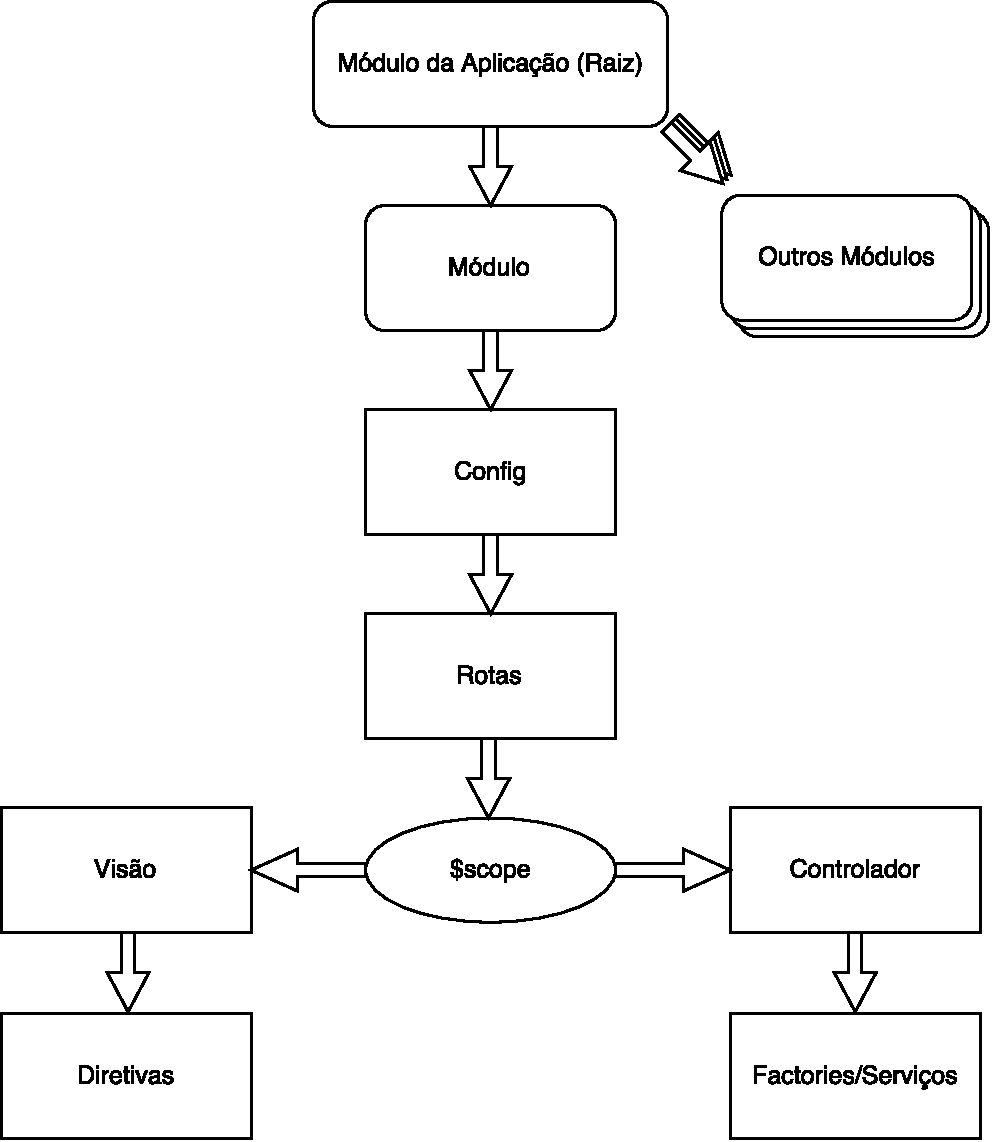
\includegraphics[scale=0.65]{5_4.pdf}
    \caption{Arquitetura de uma aplicação AngularJS \cite{website:angularjs}}
    \label{angularjs}%
\end{figure}




				

				
			
		


